\documentclass{article}
\usepackage{pinlabel}

% Nathan's basic label overlay environment.   The usual version is the second one
% below.  Args are: coor system, graphics modifiers, graphics name

\usepackage[all, import]{xy}
\newenvironment{xyoverpic}[3]
{%
\begin{xy}
\xyimport#1{\includegraphics[#2]{#3}}
}{\end{xy}}

\newenvironment{cxyoverpic}[3]
{%
\centering \leavevmode
\begin{xyoverpic}{#1}{#2}{#3}
}{\end{xyoverpic}}

\begin{document}
\begin{figure}[htb]
\labellist
\small\hair 2pt
 \pinlabel {$a$} [] at 265 117
 \pinlabel {$b$} [] at 45 195
 \pinlabel {$c$} [] at 89 159
 \pinlabel {$d$} [] at 45 127
 \pinlabel {$e$} [] at 90 90
 \pinlabel {$f$} [] at 66 28
\endlabellist
\centering
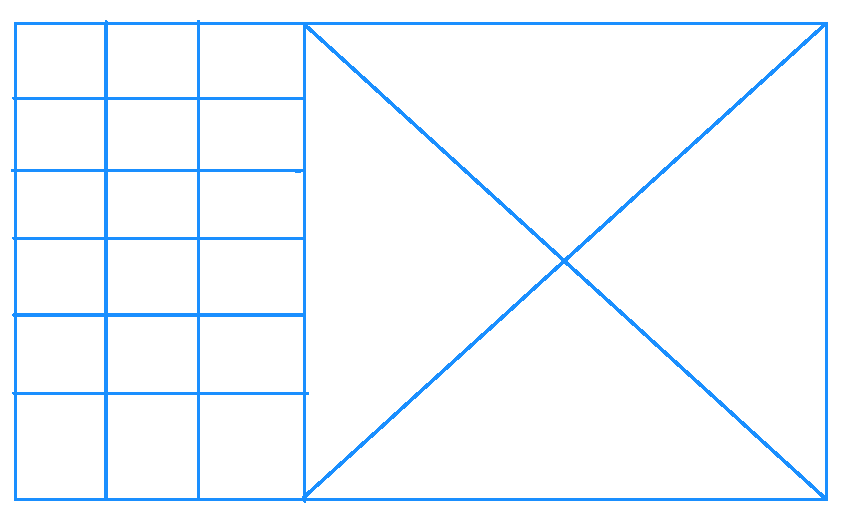
\includegraphics[scale=1.0]{test-image}
\caption{  }
\label{fig:label}
\end{figure}

\begin{figure}[htb]
\begin{cxyoverpic}{(404,250)}{scale=1.0}{test-image}
    ,(271,125)*{a}
    ,(51,203)*{b}
    ,(95,168)*{c}
    ,(51,136)*{d}
    ,(95,99)*{e}
    ,(72,36)*{f}
\end{cxyoverpic}
  \caption{}
  \label{fig-}
\end{figure}



\end{document}